\documentclass[aspectratio=169]{beamer}

\usetheme{Madrid}
\usecolortheme{seahorse}
\setbeamertemplate{navigation symbols}{}
\setbeamertemplate{footline}[frame number]

\usepackage{amsmath}
\usepackage{tikz}
\usetikzlibrary{arrows.meta,positioning}

\title[Research Introduction]{Incremental Data-Driven Robust Crew Pairing Optimization}
\subtitle{Under Evolving Uncertainty}
\author{Xinyu HUANG}
\institute{The Hong Kong Polytechnic University}
\date{}

\begin{document}

% Parole:
% Good morning everyone. My name is Xinyu HUANG. Today I will introduce my
% research project, titled Incremental Data-Driven Robust Crew Pairing
% Optimization Under Evolving Uncertainty. This is an introduction, so I will
% focus on the background, motivation, related literature, research gap, and the
% objective of my project.
\begin{frame}
  \titlepage
  \vspace{-0.35cm}
  \begin{center}
    \small Background $\rightarrow$ Literature $\rightarrow$ Research gap $\rightarrow$ Objective
  \end{center}
\end{frame}

% Parole:
% Airline crew pairing is a core planning problem in airline operations. A crew
% pairing is a sequence of flights assigned to a crew group. The airline must
% cover every flight while respecting operational rules, such as duty time, rest
% time, and connection feasibility. At the same time, the airline wants to
% control cost. This makes crew pairing a large-scale optimization problem.
\begin{frame}{Background: Crew Pairing}
  \begin{columns}[T,onlytextwidth]
    \column{0.48\textwidth}
      \textbf{What is crew pairing?}
      \begin{itemize}
        \item Assign crews to sequences of flights.
        \item Cover every flight exactly once.
        \item Respect crew duty and rest rules.
      \end{itemize}

    \column{0.48\textwidth}
      \textbf{Why is it important?}
      \begin{itemize}
        \item Crew cost is a major airline cost.
        \item Feasible schedules support daily operations.
        \item Disruptions can quickly affect later flights.
      \end{itemize}
  \end{columns}

  \vspace{0.35cm}
  \begin{block}{Core planning question}
    How can an airline design crew pairings that are low-cost and operationally reliable?
  \end{block}
\end{frame}

% Parole:
% The main difficulty is uncertainty. In real operations, flights may be delayed
% by weather, airport congestion, aircraft issues, or other unexpected events.
% A delay does not only affect one flight. It may make the crew miss the next
% connection, which creates extra recovery actions such as waiting, swapping, or
% cancellation. Therefore, a schedule that is optimal in the planning stage may
% perform badly during real operations.
\begin{frame}{Motivation: Delay Uncertainty}
  \begin{center}
  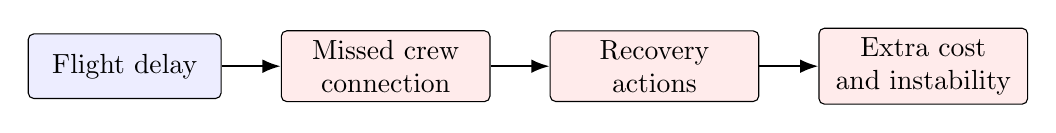
\begin{tikzpicture}[
    box/.style={draw, rounded corners=2pt, align=center, minimum width=2.45cm,
      minimum height=0.82cm, fill=blue!7},
    warn/.style={draw, rounded corners=2pt, align=center, minimum width=2.65cm,
      minimum height=0.82cm, fill=red!8},
    arrow/.style={-Latex, thick}
  ]
    \node[box] (flight) {Flight delay};
    \node[warn, right=0.75cm of flight] (miss) {Missed crew\\connection};
    \node[warn, right=0.75cm of miss] (recover) {Recovery\\actions};
    \node[warn, right=0.75cm of recover] (cost) {Extra cost\\and instability};
    \draw[arrow] (flight) -- (miss);
    \draw[arrow] (miss) -- (recover);
    \draw[arrow] (recover) -- (cost);
  \end{tikzpicture}
  \end{center}

  \vspace{0.25cm}
  \begin{itemize}
    \item Delay uncertainty can break planned crew connections.
    \item Recovery may require waiting, swapping, or cancellation.
    \item Robustness is needed, not only nominal cost minimization.
  \end{itemize}
\end{frame}

% Parole:
% The related literature has three main streams. First, robust optimization
% provides tools to protect decisions against uncertainty. The work of Bertsimas
% and Sim is important because it introduces the budget-of-uncertainty idea.
% Second, two-stage robust optimization and column-and-constraint generation
% provide solution methods for problems with recourse decisions. Third, crew
% pairing and airline recovery studies show that airline planning requires
% decomposition methods such as column generation. However, less attention has
% been paid to data-driven uncertainty sets that evolve over time and to
% incremental re-optimization for crew pairing.
\begin{frame}{Related Literature}
  \begin{columns}[T,onlytextwidth]
    \column{0.32\textwidth}
      \textbf{Robust optimization}
      \begin{itemize}
        \item Budgeted uncertainty.
        \item Robustness-cost trade-off.
        \item Bertsimas and Sim (2004).
      \end{itemize}

    \column{0.32\textwidth}
      \textbf{Two-stage methods}
      \begin{itemize}
        \item Recourse after uncertainty.
        \item Column-and-constraint generation.
        \item Zhao and Zeng (2012); Zeng and Zhao (2013).
      \end{itemize}

    \column{0.32\textwidth}
      \textbf{Transportation planning}
      \begin{itemize}
        \item Robust network and airline recovery.
        \item Column generation for large pairing spaces.
        \item Wang and Qi (2020).
      \end{itemize}
  \end{columns}
\end{frame}

% Parole:
% Based on this literature, I identify three research gaps. First, many
% uncertainty models rely on fixed assumptions or fitted distributions, which
% may underestimate rare disruptions. Second, delay uncertainty is naturally
% one-sided, because late arrivals are harmful but early arrivals are usually
% not. Third, most optimization models are solved from scratch when the data
% change, but in practice airline data are updated continuously. These gaps
% motivate my research.
\begin{frame}{Research Gap}
  \begin{enumerate}
    \item \textbf{Distributional assumptions may be fragile.}
      Rare delay events can be diluted by many normal observations.
    \item \textbf{Delay uncertainty is asymmetric.}
      Late arrivals create operational risk; early arrivals are usually absorbed.
    \item \textbf{Uncertainty evolves over time.}
      New data should update the model without rebuilding everything from zero.
  \end{enumerate}

  \vspace{0.25cm}
  \begin{block}{Gap addressed by this project}
    A data-driven robust crew pairing framework with incremental re-optimization under evolving uncertainty.
  \end{block}
\end{frame}

% Parole:
% The research objective is to design a robust and adaptive crew pairing
% optimization framework. The first idea is to construct delay bounds directly
% from historical data, using empirical quantiles. The second idea is to use a
% budget-of-uncertainty mechanism to avoid over-conservatism. The third idea is
% to keep the model updateable, so that when new data arrive, we can add
% necessary cuts and re-optimize from the previous model.
\begin{frame}{Research Objective And Direction}
  \begin{block}{Objective}
    Develop a crew pairing optimization framework that is robust, data-driven, and adaptive to new delay data.
  \end{block}

  \vspace{0.2cm}
  \begin{itemize}
    \item Use empirical quantiles to construct delay bounds:
      \[
        d_f = \mathrm{Quantile}_{\alpha}(x_f^1, x_f^2, \ldots, x_f^T)
      \]
    \item Use budgeted uncertainty to balance protection and cost.
    \item Reuse previous solutions and constraints when uncertainty changes.
  \end{itemize}
\end{frame}

% Parole:
% The expected contribution is not only a mathematical model, but also a
% practical update mechanism. The model considers both planning and recovery.
% The data-driven uncertainty set is easier to update when new delay data arrive.
% The incremental re-optimization idea can reduce repeated work because the
% algorithm does not need to restart from the beginning every time uncertainty
% changes.
\begin{frame}{Expected Contribution}
  \begin{itemize}
    \item \textbf{Modeling contribution:}
      quantile-based, one-sided uncertainty set for delay disruptions.
    \item \textbf{Optimization contribution:}
      two-stage robust crew pairing with recovery actions.
    \item \textbf{Algorithmic contribution:}
      nested C\&CG and column generation for large-scale solution.
    \item \textbf{Practical contribution:}
      incremental re-optimization as delay information evolves.
  \end{itemize}
\end{frame}

% Parole:
% To conclude, this project starts from an important airline planning problem:
% crew pairing under delay uncertainty. The related literature provides useful
% tools from robust optimization, two-stage optimization, and column generation.
% However, evolving data-driven uncertainty has not been fully addressed in this
% context. My project aims to fill this gap by combining quantile-based delay
% bounds, budgeted robustness, and incremental re-optimization. Thank you for
% listening.
\begin{frame}{Conclusion}
  \begin{itemize}
    \item Crew pairing is cost-sensitive and operationally critical.
    \item Delay uncertainty can make nominal schedules unreliable.
    \item Related literature motivates robust, two-stage, and decomposition-based methods.
    \item This project focuses on data-driven uncertainty and incremental model updates.
  \end{itemize}

  \vspace{0.3cm}
  \begin{block}{Final message}
    The project introduces a robust crew pairing framework that can learn from delay data and adapt as uncertainty evolves.
  \end{block}
\end{frame}

\end{document}
